\documentclass{standalone}
\usepackage{tikz}
\usetikzlibrary{patterns, positioning}
\usepackage[sfdefault]{ClearSans} %% option 'sfdefault' activates Clear Sans as the default text font
\usepackage[T1]{fontenc}

\begin{document}
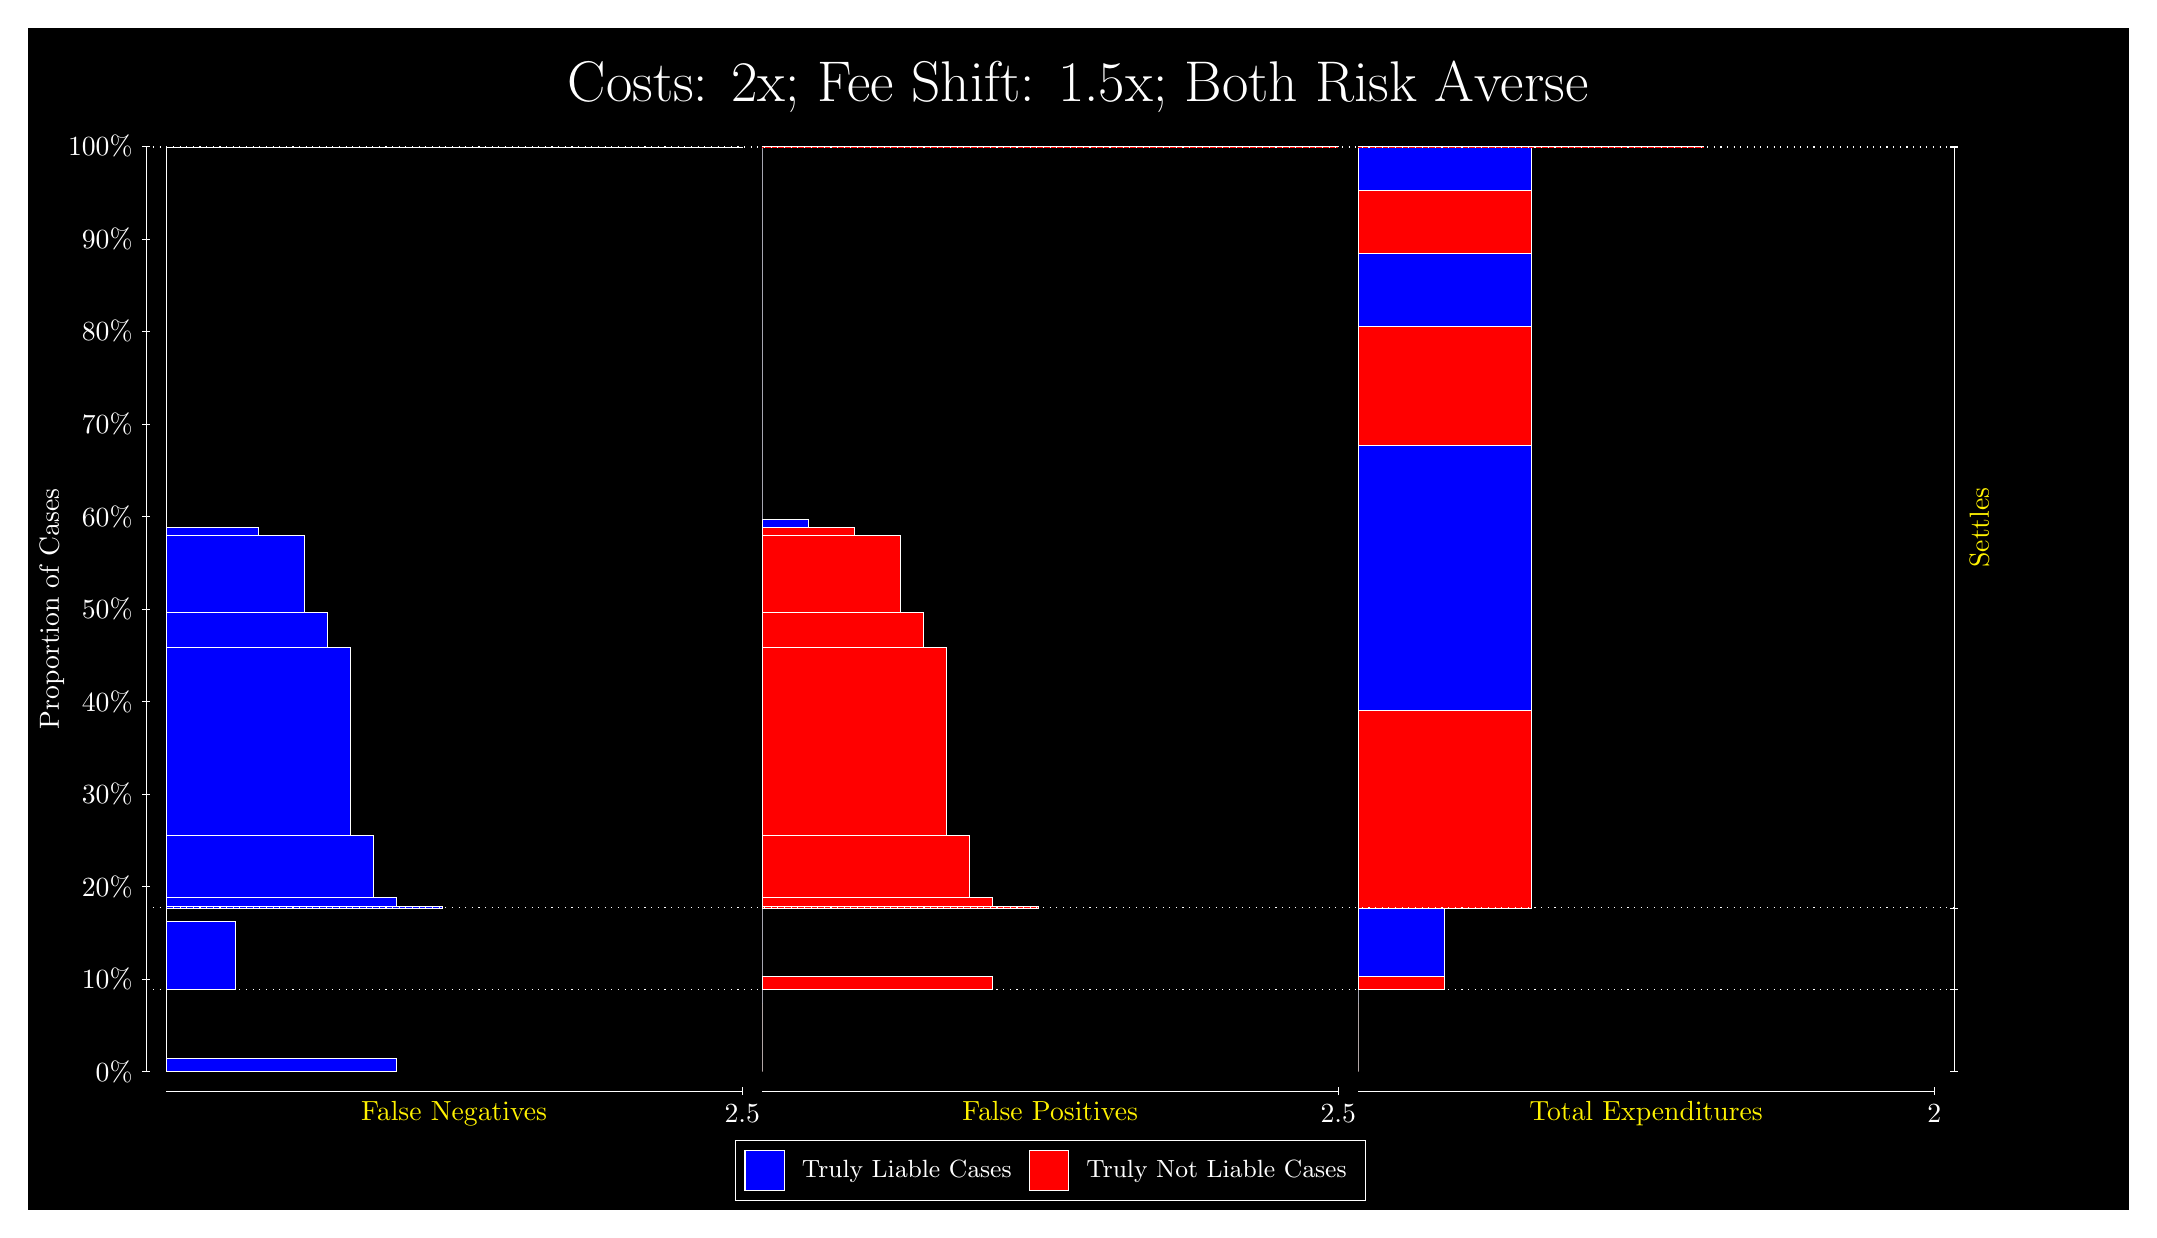
\begin{tikzpicture}
\draw[fill=black] (0,0) rectangle (26.667,15);
\draw[text=white] (0,13.5) rectangle (26.667,15) node[midway] {\huge Costs: 2x; Fee Shift: 1.5x; Both Risk Averse};
\draw[white, very thin] (1.5,1.75) -- (1.5,13.5);
\node[rotate=90, text=white, anchor=center] at (0.3, 7.625) {Proportion of Cases};
\draw[white, very thin] (1.45,1.75) -- (1.55,1.75);
\node[text=white, anchor=east] at (1.45, 1.75) {0\%};
\draw[white, very thin] (1.45,2.925) -- (1.55,2.925);
\node[text=white, anchor=east] at (1.45, 2.925) {10\%};
\draw[white, very thin] (1.45,4.1) -- (1.55,4.1);
\node[text=white, anchor=east] at (1.45, 4.1) {20\%};
\draw[white, very thin] (1.45,5.275) -- (1.55,5.275);
\node[text=white, anchor=east] at (1.45, 5.275) {30\%};
\draw[white, very thin] (1.45,6.45) -- (1.55,6.45);
\node[text=white, anchor=east] at (1.45, 6.45) {40\%};
\draw[white, very thin] (1.45,7.625) -- (1.55,7.625);
\node[text=white, anchor=east] at (1.45, 7.625) {50\%};
\draw[white, very thin] (1.45,8.8) -- (1.55,8.8);
\node[text=white, anchor=east] at (1.45, 8.8) {60\%};
\draw[white, very thin] (1.45,9.975) -- (1.55,9.975);
\node[text=white, anchor=east] at (1.45, 9.975) {70\%};
\draw[white, very thin] (1.45,11.15) -- (1.55,11.15);
\node[text=white, anchor=east] at (1.45, 11.15) {80\%};
\draw[white, very thin] (1.45,12.325) -- (1.55,12.325);
\node[text=white, anchor=east] at (1.45, 12.325) {90\%};
\draw[white, very thin] (1.45,13.5) -- (1.55,13.5);
\node[text=white, anchor=east] at (1.45, 13.5) {100\%};

\draw[white, very thin] (24.457,1.75) -- (24.457,13.5);
\draw[white, very thin] (24.407,1.75) -- (24.507,1.75);
\node[anchor=west] at (24.407, 1.75) {};
\draw[white, very thin] (24.407,2.79) -- (24.507,2.79);
\node[anchor=west] at (24.407, 2.79) {};
\draw[white, very thin] (24.407,3.8296) -- (24.507,3.8296);
\node[anchor=west] at (24.407, 3.8296) {};
\draw[white, very thin] (24.407,13.489) -- (24.507,13.489);
\node[anchor=west] at (24.407, 13.489) {};
\draw[white, very thin] (24.407,13.495) -- (24.507,13.495);
\node[anchor=west] at (24.407, 13.495) {};
\draw[white, very thin] (24.407,13.5) -- (24.507,13.5);
\node[anchor=west] at (24.407, 13.5) {};

\draw[white, very thin, fill=blue] (1.75,1.75) rectangle (4.6775,1.9214);
\draw[white, very thin, fill=red] (1.75,1.9214) rectangle (1.75,2.79);
\draw[white, very thin, fill=blue] (1.75,2.79) rectangle (2.6283,3.6583);
\draw[white, very thin, fill=red] (1.75,3.6583) rectangle (1.75,3.8296);
\draw[white, very thin, fill=blue] (1.75,3.8296) rectangle (5.2631,3.851);
\draw[white, very thin, fill=blue] (1.75,3.851) rectangle (4.6775,3.9624);
\draw[white, very thin, fill=blue] (1.75,3.9624) rectangle (4.3848,4.7492);
\draw[white, very thin, fill=blue] (1.75,4.7492) rectangle (4.092,7.1421);
\draw[white, very thin, fill=blue] (1.75,7.1421) rectangle (3.7993,7.5821);
\draw[white, very thin, fill=blue] (1.75,7.5821) rectangle (3.5065,8.5565);
\draw[white, very thin, fill=blue] (1.75,8.5565) rectangle (2.921,8.6594);
\draw[white, very thin, fill=red] (1.75,8.6594) rectangle (1.75,13.489);
\draw[white, very thin, fill=blue] (1.75,13.489) rectangle (9.0689,13.491);
\draw[white, very thin, fill=red] (1.75,13.491) rectangle (1.75,13.495);
\draw[white, very thin, fill=red] (1.75,13.495) rectangle (1.75,13.497);
\draw[white, very thin, fill=blue] (1.75,13.497) rectangle (1.75,13.5);
\draw[white, very thin, fill=red] (9.3189,1.75) rectangle (9.3189,2.6186);
\draw[white, very thin, fill=blue] (9.3189,2.6186) rectangle (9.3189,2.79);
\draw[white, very thin, fill=red] (9.3189,2.79) rectangle (12.246,2.9612);
\draw[white, very thin, fill=blue] (9.3189,2.9612) rectangle (9.3189,3.8296);
\draw[white, very thin, fill=red] (9.3189,3.8296) rectangle (12.832,3.851);
\draw[white, very thin, fill=red] (9.3189,3.851) rectangle (12.246,3.9624);
\draw[white, very thin, fill=red] (9.3189,3.9624) rectangle (11.954,4.7493);
\draw[white, very thin, fill=red] (9.3189,4.7493) rectangle (11.661,7.1423);
\draw[white, very thin, fill=red] (9.3189,7.1423) rectangle (11.368,7.582);
\draw[white, very thin, fill=red] (9.3189,7.582) rectangle (11.075,8.5565);
\draw[white, very thin, fill=red] (9.3189,8.5565) rectangle (10.49,8.6594);
\draw[white, very thin, fill=blue] (9.3189,8.6594) rectangle (9.9044,8.7623);
\draw[white, very thin, fill=blue] (9.3189,8.7623) rectangle (9.3189,13.489);
\draw[white, very thin, fill=red] (9.3189,13.489) rectangle (9.3189,13.493);
\draw[white, very thin, fill=blue] (9.3189,13.493) rectangle (9.3189,13.495);
\draw[white, very thin, fill=red] (9.3189,13.495) rectangle (16.638,13.497);
\draw[white, very thin, fill=blue] (9.3189,13.497) rectangle (13.71,13.5);
\draw[white, very thin, fill=red] (16.888,1.75) rectangle (16.888,2.6186);
\draw[white, very thin, fill=blue] (16.888,2.6186) rectangle (16.888,2.79);
\draw[white, very thin, fill=red] (16.888,2.79) rectangle (17.986,2.9612);
\draw[white, very thin, fill=blue] (16.888,2.9612) rectangle (17.986,3.8296);
\draw[white, very thin, fill=red] (16.888,3.8296) rectangle (19.083,6.3338);
\draw[white, very thin, fill=blue] (16.888,6.3338) rectangle (19.083,9.7011);
\draw[white, very thin, fill=red] (16.888,9.7011) rectangle (19.083,11.218);
\draw[white, very thin, fill=blue] (16.888,11.218) rectangle (19.083,12.138);
\draw[white, very thin, fill=red] (16.888,12.138) rectangle (19.083,12.946);
\draw[white, very thin, fill=blue] (16.888,12.946) rectangle (19.083,13.489);
\draw[white, very thin, fill=red] (16.888,13.489) rectangle (21.279,13.493);
\draw[white, very thin, fill=blue] (16.888,13.493) rectangle (21.279,13.495);
\draw[white, very thin, fill=red] (16.888,13.495) rectangle (21.279,13.497);
\draw[white, very thin, fill=blue] (16.888,13.497) rectangle (21.279,13.5);
\draw[white, dotted] (1.5,2.79) -- (24.457,2.79);
\draw[white, dotted] (1.5,3.8296) -- (24.457,3.8296);
\draw[white, dotted] (1.5,13.489) -- (24.457,13.489);
\draw[white, dotted] (1.5,13.495) -- (24.457,13.495);
\draw[white, very thin] (1.75,1.5) -- (9.0689,1.5);
\node[text=yellow, anchor=north] at (5.4094, 1.5) {False Negatives};
\draw[white, very thin] (9.0689,1.45) -- (9.0689,1.55);
\node[text=white, anchor=north] at (9.0689, 1.45) {2.5};

\draw[white, very thin] (9.3189,1.5) -- (16.638,1.5);
\node[text=yellow, anchor=north] at (12.978, 1.5) {False Positives};
\draw[white, very thin] (16.638,1.45) -- (16.638,1.55);
\node[text=white, anchor=north] at (16.638, 1.45) {2.5};

\draw[white, very thin] (16.888,1.5) -- (24.207,1.5);
\node[text=yellow, anchor=north] at (20.547, 1.5) {Total Expenditures};
\draw[white, very thin] (24.207,1.45) -- (24.207,1.55);
\node[text=white, anchor=north] at (24.207, 1.45) {2};



\node[text=yellow, centered, rotate=90] at (24.777, 8.6594) {Settles};



\draw (12.978300999999998,1.5) node[draw=none] (baseCoordinate) {};
\begin{scope}[align=center]
        \matrix[scale=0.5, draw=white, below=0.5cm of baseCoordinate, nodes={draw}, column sep=0.1cm]{
            \node[rectangle, draw, minimum width=0.5cm, minimum height=0.5cm, fill=blue] {}; &
            \node[draw=none, font=\small, text=white] (B) {Truly Liable Cases}; &
            \node[rectangle, draw, minimum width=0.5cm, minimum height=0.5cm, fill=red] {}; &
            \node[draw=none, font=\small, text=white] (B) {Truly Not Liable Cases}; \\
            };
\end{scope}

\end{tikzpicture}
\end{document}